\chapter{Effective Thermal History, Production-Surface Matching, Reionization, and Late-Time Line-of-Sight Closure}
\label{ch:thermal-reionization-los}

\section{Scope and objective}

The preceding production-to-primary-CMB calculation jointly evolved photons, scalar polarization, baryons, massless neutrinos, metric perturbations, and the massive refinement hierarchy through a controlled recombination surface.  Its stated thermal and projection limitations were Saha hydrogen recombination, no reionization, no late integrated Sachs--Wolfe source, and a narrow finite-width last-scattering projection.  This chapter extends that framework by adding
\begin{equation}
\boxed{
\begin{gathered}
\text{effective Peebles hydrogen recombination}
+\text{ controlled helium transitions}\\
+\text{ optical-depth-calibrated reionization}
+\text{ single-clock production matching}\\
+\text{ finite-width recombination and reionization projection}
+\text{ time-resolved late ISW transport}.
\end{gathered}}
\label{eq:trl-objective}
\end{equation}
The early acoustic source amplitudes are inherited from the coupled Einstein--Boltzmann solve without dark-sector retuning.  The new calculation is a controlled thermal-history and late-source closure.  It is not a precision recombination code, an astrophysical reionization prediction, or a likelihood analysis.

A sign correction is also made.  In the Newtonian-gauge convention used here, the integrated temperature source is proportional to
\begin{equation}
\Phi'+\Psi',
\label{eq:trl-isw-sum}
\end{equation}
not to their difference.  The corrected sum is used throughout this chapter.

\section{Unchanged cosmological and refinement input}

Use
\begin{equation}
E(a)^2
=
\Omega_{r0}a^{-4}
+\Omega_{m0}a^{-3}
+\Omega_{V0},
\qquad
\Omega_{m0}=\Omega_{b0}+\Omega_{D0},
\label{eq:trl-background}
\end{equation}
with
\begin{equation}
\Omega_{b0}=0.049,
\qquad
\Omega_{D0}=0.261,
\qquad
\Omega_{r0}=9\times10^{-5},
\qquad
\Omega_{V0}=1-\Omega_{m0}-\Omega_{r0}.
\label{eq:trl-fractions}
\end{equation}
The conditional physical conversion uses
\begin{equation}
H_0=70\ {\rm km\,s^{-1}\,Mpc^{-1}},
\qquad
T_{\gamma0}=2.7255\ {
m K},
\qquad
Y_p=0.24.
\label{eq:trl-conventions}
\end{equation}
The primordial spectrum remains
\begin{equation}
\mathcal P_{\mathcal R}(k)
=A_s\left(\frac{k}{k_\star}\right)^{n_s-1},
\qquad
A_s=2.1\times10^{-9},
\qquad
n_s=0.965,
\qquad
k_\star=0.05\ {\rm Mpc}^{-1}.
\label{eq:trl-primordial}
\end{equation}
The recombination-era acoustic source functions
\begin{equation}
A_T(k),\qquad A_V(k),\qquad A_E(k)
\label{eq:trl-parent-sources}
\end{equation}
are read directly from the preceding coupled solve.  No parameter of the scale-covariant dark sector is refitted in this calculation.

\section{Effective Peebles hydrogen recombination}

Let
\begin{equation}
N=\log a,
\qquad
T_\gamma=\frac{T_{\gamma0}}{a},
\qquad
n_H(a)=n_{H0}a^{-3}.
\label{eq:trl-recomb-definitions}
\end{equation}
The case-B coefficient is represented by the controlled fit
\begin{equation}
\alpha_B(T)
=
4.309\times10^{-19}
\frac{t^{-0.6166}}{1+0.6703t^{0.5300}}
\ {\rm m^3\,s^{-1}},
\qquad
t=\frac{T}{10^4\ {\rm K}}.
\label{eq:trl-alphaB}
\end{equation}
Detailed balance gives
\begin{equation}
\beta_B(T)
=
\alpha_B(T)
\left(\frac{m_ek_BT}{2\pi\hbar^2}\right)^{3/2}
\exp\left(-\frac{E_2}{k_BT}\right),
\qquad
E_2=3.4\ {\rm eV}.
\label{eq:trl-betaB}
\end{equation}
Define
\begin{equation}
K_\alpha
=
\frac{\lambda_\alpha^3}{8\pi H},
\qquad
C_P
=
\frac{1+K_\alpha\Lambda_{2s}n_H(1-x_H)}
{1+K_\alpha(\Lambda_{2s}+\beta_B)n_H(1-x_H)}.
\label{eq:trl-peebles-C}
\end{equation}
The effective three-level hydrogen equation is
\begin{equation}
\boxed{
\frac{dx_H}{dN}
=
\frac{C_P}{H}
\left[
\beta_B(1-x_H)
\exp\left(-\frac{E_\alpha}{k_BT}\right)
-n_H\alpha_Bx_H^2
\right],
}
\label{eq:trl-peebles-eq}
\end{equation}
where
\begin{equation}
E_\alpha=10.2\ {\rm eV},
\qquad
\Lambda_{2s}=8.22458\ {\rm s}^{-1},
\qquad
\lambda_\alpha=121.567\ {\rm nm}.
\label{eq:trl-atomic-constants}
\end{equation}
The calculation follows the Saha solution until
\begin{equation}
x_H\simeq0.99,
\qquad
z\simeq1577.09,
\label{eq:trl-switch}
\end{equation}
and then integrates \eqref{eq:trl-peebles-eq}.  It gives
\begin{equation}
\boxed{x_{H,{\rm residual}}=2.8029283896\times10^{-4}.}
\label{eq:trl-residual-xe}
\end{equation}

The helium contribution is represented by controlled smooth transitions for HeIII-to-HeII and HeII-to-HeI.  This preserves the correct electron-counting limits but is not a multilevel helium-kinetics calculation.

\section{Reionization and optical-depth calibration}

Let
\begin{equation}
y(z)=(1+z)^{3/2}.
\label{eq:trl-yre}
\end{equation}
The hydrogen reionization fraction is modeled by
\begin{equation}
R_H(z)
=
\frac12
\left[
1+\tanh\left(
\frac{y(z_{\rm re})-y(z)}{\Delta y_{\rm re}}
\right)
\right],
\label{eq:trl-tanh-reionization}
\end{equation}
with
\begin{equation}
\Delta y_{\rm re}
=
\frac32\sqrt{1+z_{\rm re}}\,\Delta z_{\rm re},
\qquad
\Delta z_{\rm re}=0.5.
\label{eq:trl-dyre}
\end{equation}
A second smooth transition accounts for the late second helium ionization.

The optical-depth equation in logarithmic scale factor is
\begin{equation}
\frac{d\tau}{dN}
=
\frac{n_e\sigma_Tc}{H},
\label{eq:trl-tau}
\end{equation}
and the visibility per unit $N$ is
\begin{equation}
g_N(N)
=
\exp[-\tau(N)]\frac{d\tau}{dN}.
\label{eq:trl-visibility}
\end{equation}
The reionization midpoint is fixed by the declared input
\begin{equation}
\tau_{\rm re}=0.054.
\label{eq:trl-tau-target}
\end{equation}
The calibrated result is
\begin{equation}
\boxed{z_{\rm re}=7.4124651067,}
\qquad
\boxed{z_{g,{\rm re}}=6.6559660691.}
\label{eq:trl-zre-results}
\end{equation}
The total visibility satisfies
\begin{equation}
\boxed{
\int g_N\,dN
=0.9999979519.
}
\label{eq:trl-visibility-normalization}
\end{equation}
The recombination and reionization pieces carry
\begin{equation}
\int g_{N,{\rm rec}}\,dN=0.9474304116,
\qquad
\int g_{N,{\rm re}}\,dN=0.0525675402.
\label{eq:trl-vis-split}
\end{equation}

\begin{figure}[htbp]
\centering
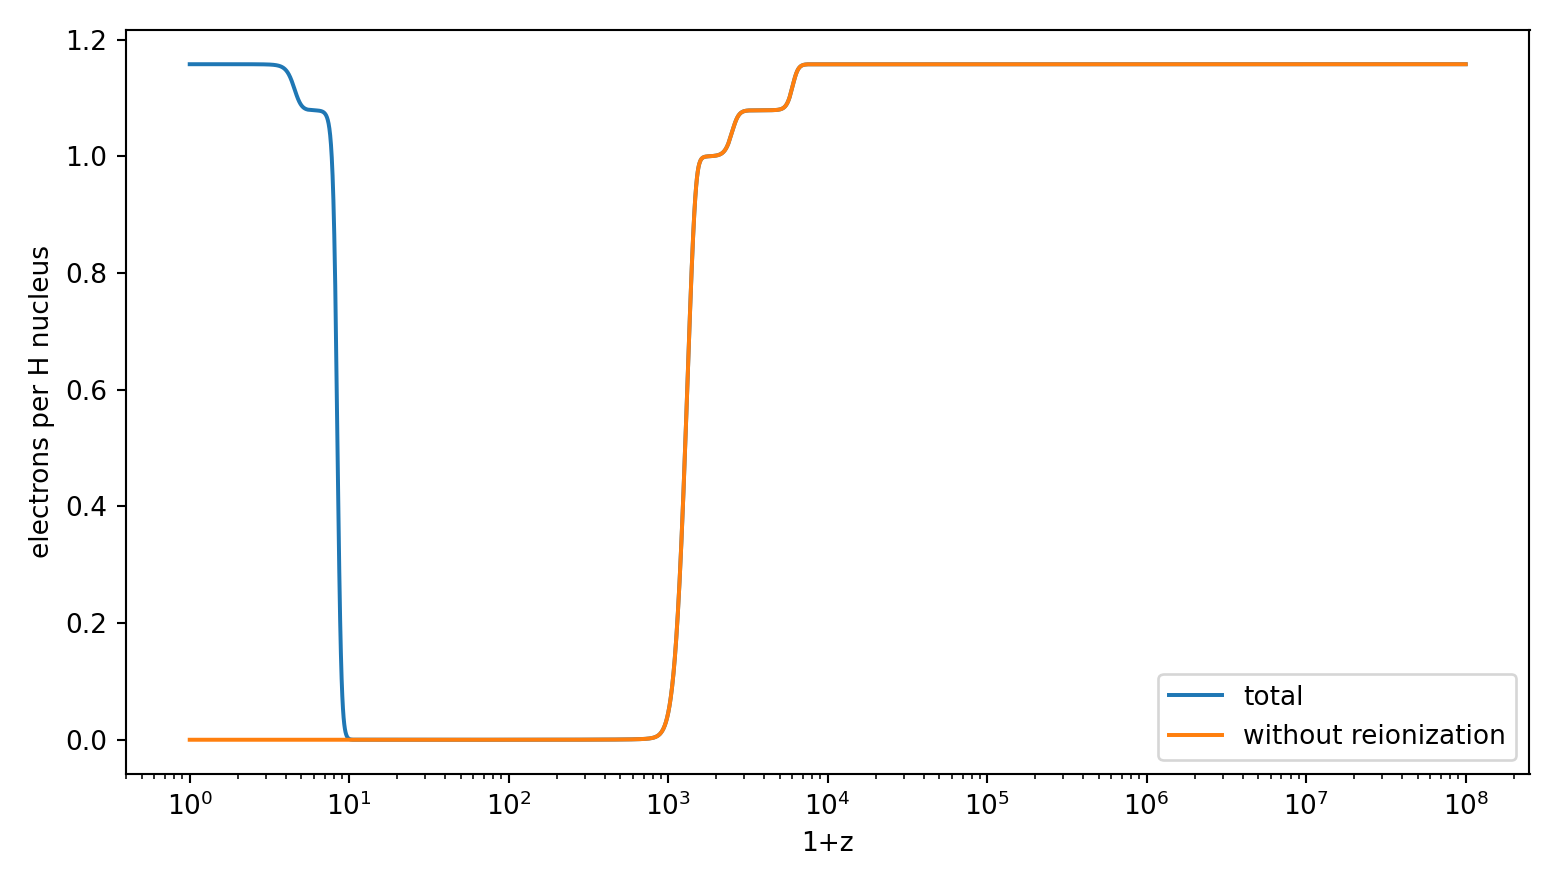
\includegraphics[width=0.86\linewidth]{figures/los/effective_ionization_history.png}
\caption{Effective hydrogen-plus-helium ionization history before and after the optical-depth-calibrated reionization transition.}
\label{fig:trl-ionization}
\end{figure}

\begin{figure}[htbp]
\centering
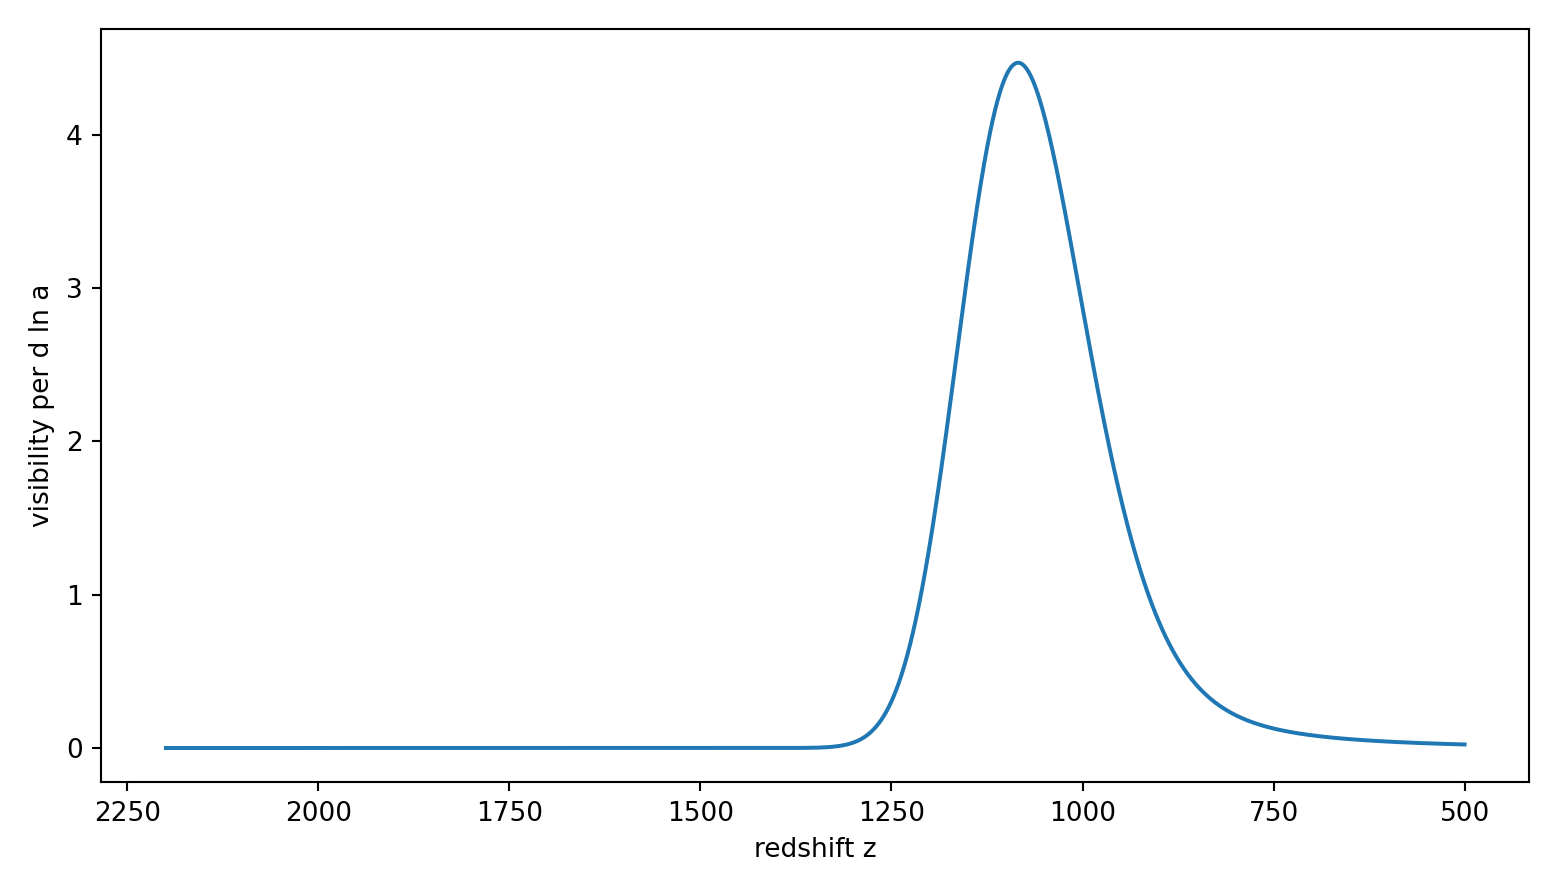
\includegraphics[width=0.82\linewidth]{figures/los/effective_recombination_visibility.png}
\caption{Effective recombination visibility.  The peak shifts from the preceding Saha benchmark to the controlled Peebles value near $z=1084$.}
\label{fig:trl-recombination-vis}
\end{figure}

\begin{figure}[htbp]
\centering
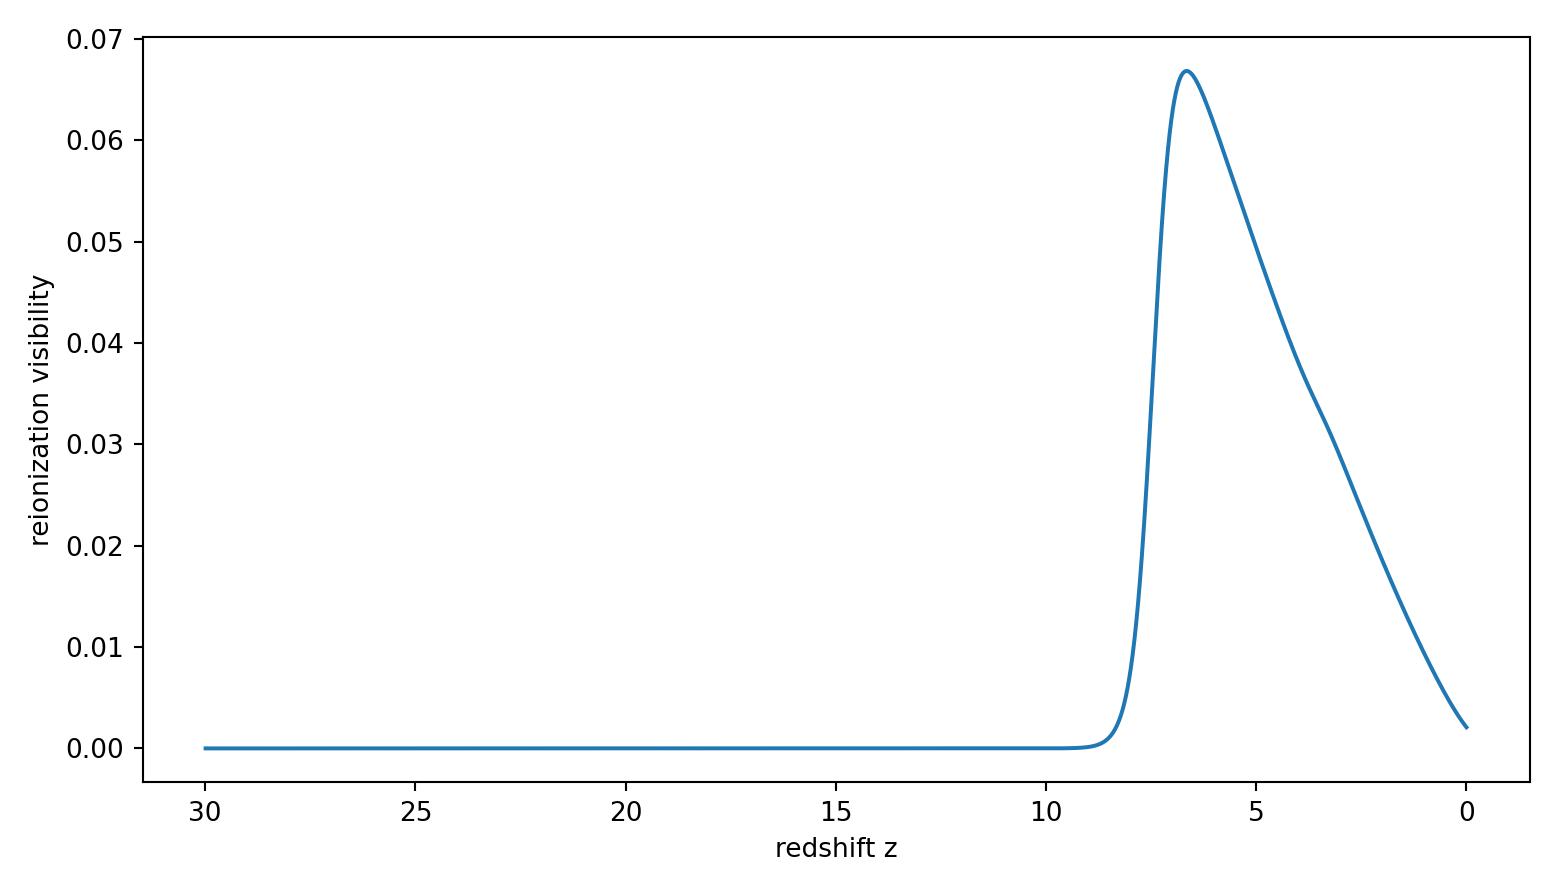
\includegraphics[width=0.82\linewidth]{figures/los/reionization_visibility.png}
\caption{Reionization-only visibility after subtracting the recombination history.}
\label{fig:trl-reionization-vis}
\end{figure}

\section{Visibility moments and finite-thickness projection}

For a nonnegative source weight $w(N)$, define
\begin{equation}
\mathcal N_w=\int w\,dN,
\qquad
\chi_w=\frac{1}{\mathcal N_w}\int w\chi\,dN,
\label{eq:trl-shell-mean}
\end{equation}
\begin{equation}
\sigma_{\chi,w}^2
=
\frac{1}{\mathcal N_w}
\int w(\chi-\chi_w)^2\,dN.
\label{eq:trl-shell-rms}
\end{equation}
The long residual-ionization tail makes the global recombination RMS width a poor Gaussian approximation to the acoustic core.  The calculation therefore archives the full visibility and both widths, while the acoustic thickness factor uses the FWHM-equivalent central width
\begin{equation}
\sigma_{\chi,{\rm core}}
=
\frac{\Delta\chi_{\rm FWHM}}{2\sqrt{2\log2}}.
\label{eq:trl-core-width}
\end{equation}
The measured quantities are
\begin{equation}
\boxed{
\chi_{\rm rec}=3.1335298685\ H_0^{-1},
\qquad
\sigma_{\chi,{\rm core}}=3.7505054558\times10^{-3}\ H_0^{-1},
}
\label{eq:trl-rec-shell}
\end{equation}
\begin{equation}
\sigma_{\chi,{\rm RMS}}=1.6282448527\times10^{-2}\ H_0^{-1},
\label{eq:trl-rec-rms}
\end{equation}
\begin{equation}
\boxed{
\chi_{\rm re}=1.5792968823\ H_0^{-1},
\qquad
\sigma_{\chi,{\rm re}}=0.4275528337\ H_0^{-1}.
}
\label{eq:trl-re-shell}
\end{equation}
The recombination visibility peaks at
\begin{equation}
\boxed{z_{\rm rec}=1084.47305577.}
\label{eq:trl-zrec}
\end{equation}

\section{Single-clock production-surface matching}

Let the production hypersurface be defined by one local clock $F$,
\begin{equation}
F(t,\boldsymbol x)=F_\star.
\label{eq:trl-production-surface}
\end{equation}
At first perturbative order, its displacement is
\begin{equation}
\delta t_\star
=-\frac{\delta F}{\dot{\bar F}}.
\label{eq:trl-deltat}
\end{equation}
Suppose every produced refinement level depends on the same clock and no independent modulation field is present.  Then
\begin{equation}
\delta\rho_h
=-\dot{\bar\rho}_h\,\delta t_\star.
\label{eq:trl-density-matching}
\end{equation}
The curvature perturbation of each level is
\begin{equation}
\zeta_h
=-\Phi-H\frac{\delta\rho_h}{\dot{\bar\rho}_h}
=-\Phi+H\delta t_\star,
\label{eq:trl-zeta-level}
\end{equation}
so that
\begin{equation}
\boxed{
S_{hj}:=3(\zeta_h-\zeta_j)=0.
}
\label{eq:trl-zero-isocurvature}
\end{equation}
Thus a single-clock crossing supplies adiabatic production-surface matching at leading gradient order.

An independent modulation $A_\star(\boldsymbol x)$ generates a calculable entropy direction.  For
\begin{equation}
n_h
\propto
\nu_h^{3/2}
\exp\left(-\frac{\pi m_h^2}{\nu_h}\right),
\qquad
\nu_h=A_\star m_h,
\label{eq:trl-number-spectrum}
\end{equation}
its response is
\begin{equation}
\boxed{
\frac{\partial\log n_h}{\partial\log A_\star}
=
\frac32+\frac{\pi m_h}{A_\star}.
}
\label{eq:trl-modulation-response}
\end{equation}
This distinguishes the adiabatic single-clock prediction from an independently modulated production event.

\begin{figure}[htbp]
\centering
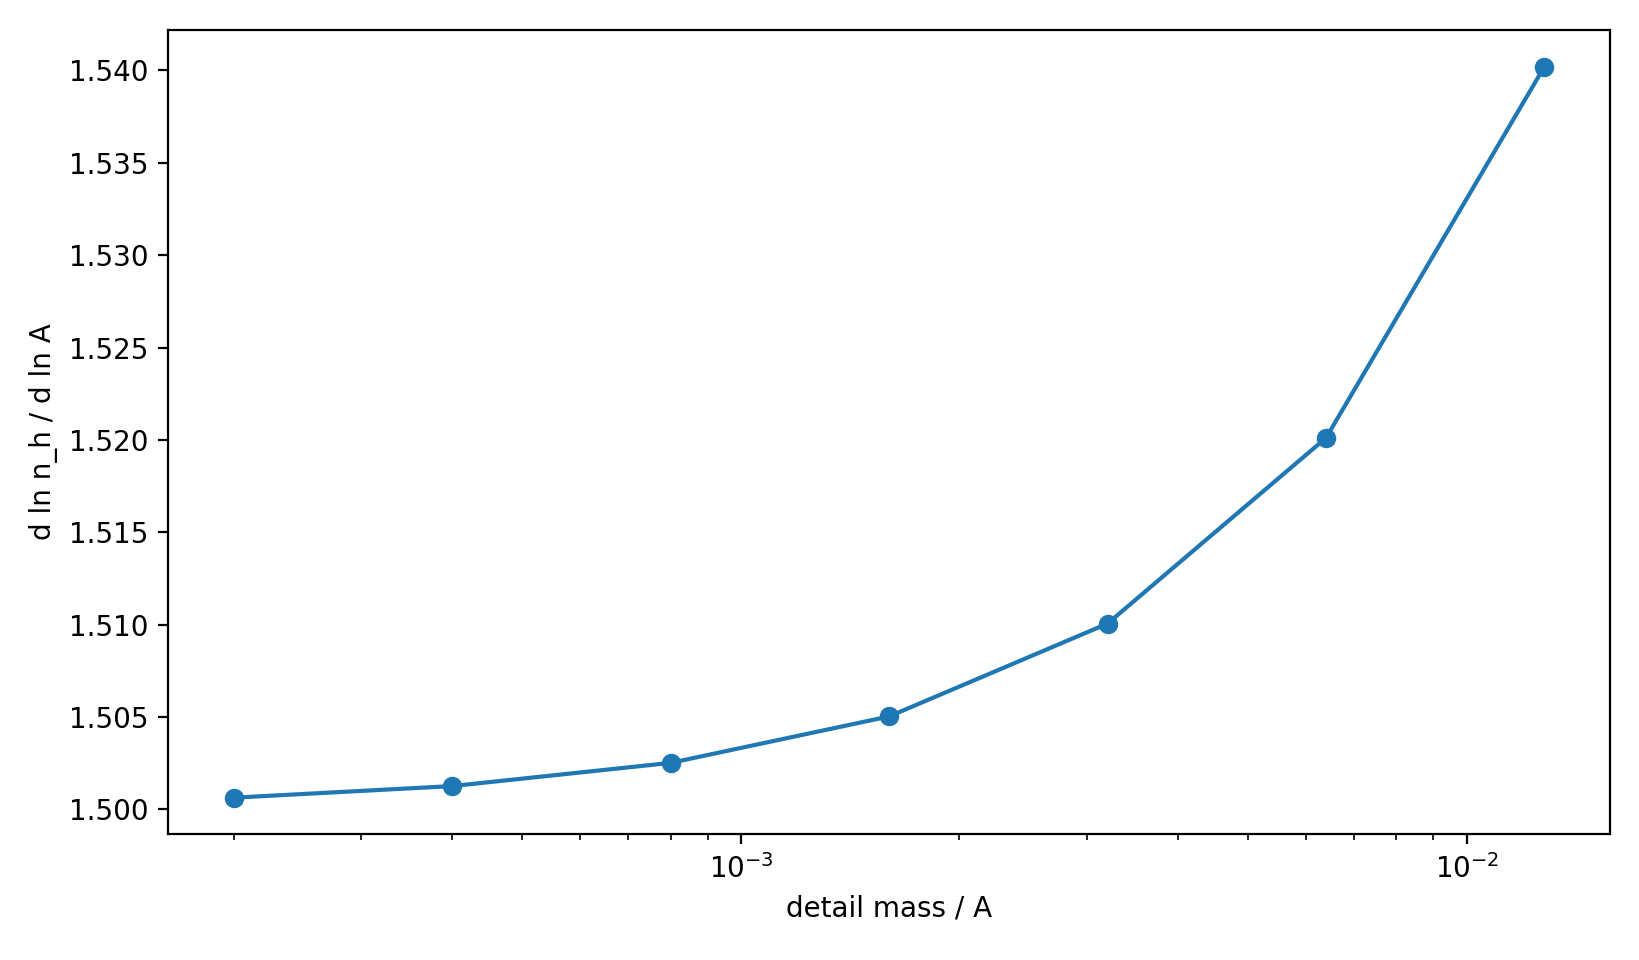
\includegraphics[width=0.80\linewidth]{figures/los/production_modulation_response.png}
\caption{Level-dependent abundance response to an independent production-scale modulation.  The single-clock relative entropy remains zero; the plotted response applies only to an additional modulation direction.}
\label{fig:trl-production-response}
\end{figure}

\section{Corrected line-of-sight source}

Use Newtonian gauge
\begin{equation}
ds^2
=a^2(\eta)
\left[-(1+2\Psi)d\eta^2+(1-2\Phi)d\boldsymbol x^2\right].
\label{eq:trl-newtonian-gauge}
\end{equation}
For the collisionless temperature brightness after the standard gravitational redshift rearrangement,
\begin{equation}
(\Theta+\Psi)'
+ik\mu(\Theta+\Psi)
=
\Phi'+\Psi'+\mathcal C_\gamma.
\label{eq:trl-los-eq}
\end{equation}
Therefore the late integrated source is
\begin{equation}
\boxed{
S_{\rm ISW}=e^{-\tau}(\Phi'+\Psi').
}
\label{eq:trl-isw-source}
\end{equation}
The earlier difference source is superseded in this convention.

Let
\begin{equation}
\mathcal T_\ell(k)
=\mathcal T_{\ell,{\rm rec}}(k)
+\mathcal T_{\ell,{\rm re}}(k)
+\mathcal T_{\ell,{\rm ISW}}(k).
\label{eq:trl-total-transfer}
\end{equation}
The finite-width recombination term is
\begin{equation}
\mathcal T_{\ell,{\rm rec}}
=e^{-\tau_{\rm re}}
\exp\left(-\frac{k^2\sigma_{\chi,{\rm core}}^2}{2}\right)
\left[
A_T(k)j_\ell(k\chi_{\rm rec})
+A_V(k)j_\ell'(k\chi_{\rm rec})
\right].
\label{eq:trl-rec-transfer}
\end{equation}
Free streaming from recombination to the effective reionization shell reconstructs
\begin{equation}
\Theta_0^{\rm re}(k)
=A_Tj_0(k\Delta\chi)+A_Vj_0'(k\Delta\chi),
\label{eq:trl-reion-monopole}
\end{equation}
\begin{equation}
\Theta_2^{\rm re}(k)
=A_Tj_2(k\Delta\chi)+A_Vj_2'(k\Delta\chi),
\qquad
\Pi_{\rm re}=4\Theta_2^{\rm re},
\label{eq:trl-reion-quadrupole}
\end{equation}
where
\begin{equation}
\Delta\chi=\chi_{\rm rec}-\chi_{\rm re}.
\label{eq:trl-deltachi}
\end{equation}
The reionization temperature and polarization sources are then projected with the measured reionization width.

The late potential is evolved with
\begin{equation}
D_{NN}
+\left(2+\frac{d\log H}{dN}\right)D_N
-\frac32\Omega_m(a)D=0,
\label{eq:trl-growth}
\end{equation}
\begin{equation}
g_\Phi(a)=\frac{D(a)}{a},
\qquad
\Phi=\Psi=\frac35\mathcal R\,T(k)g_\Phi(a),
\label{eq:trl-potential-growth}
\end{equation}
which gives the time-resolved integral
\begin{equation}
\mathcal T_{\ell,{\rm ISW}}(k)
=
\int dN\,
2e^{-\tau}
\frac{d\Phi}{dN}
 j_\ell[k\chi(N)].
\label{eq:trl-isw-integral}
\end{equation}
The $E$-mode transfer is constructed from the recombination and reionization quadrupole sources with the scalar spin-2 projection factor
\begin{equation}
\sqrt{\frac{(\ell+2)!}{(\ell-2)!}}
\frac{j_\ell(x)}{x^2}.
\label{eq:trl-spin2}
\end{equation}
Finally,
\begin{equation}
\boxed{
C_\ell^{XY}
=4\pi\int d\log k\,
\mathcal P_{\mathcal R}(k)
\mathcal T_\ell^X(k)
\mathcal T_\ell^Y(k),
\qquad
X,Y\in\{T,E\}.
}
\label{eq:trl-cl}
\end{equation}

\section{Acoustic ruler and controlled spectra}

The effective sound horizon is
\begin{equation}
r_s
=\int^{N_{\rm rec}}
\frac{dN}{\mathcal H\sqrt{3(1+R_b)}},
\qquad
R_b=\frac{3\rho_b}{4\rho_\gamma}.
\label{eq:trl-rs}
\end{equation}
The calculation gives
\begin{equation}
\boxed{H_0r_s=0.03280490608,}
\qquad
\boxed{\ell_A=\frac{\pi\chi_{\rm rec}}{r_s}=300.0854321.}
\label{eq:trl-acoustic-ruler}
\end{equation}
The first three resolved temperature maxima above $\ell=150$ occur at
\begin{equation}
\boxed{
\ell_1=262,
\qquad
\ell_2=582,
\qquad
\ell_3=894.
}
\label{eq:trl-peaks}
\end{equation}
The first peak amplitude is
\begin{equation}
\boxed{D_{262}^{TT}=4063.713734\ \mu{\rm K}^2.}
\label{eq:trl-first-peak}
\end{equation}

\begin{table}[htbp]
\centering
\small
\begin{tabular}{rrrr}
\toprule
$\ell$ & $D_\ell^{TT}$ [$\mu{\rm K}^2$] & $D_\ell^{EE}$ [$\mu{\rm K}^2$] & $D_\ell^{TE}$ [$\mu{\rm K}^2$]\\
\midrule
2    & 316.421 & 0.03564 & 1.6379\\
5    & 317.116 & 0.00992 & 0.9739\\
10   & 396.325 & 0.00006 & 0.1210\\
50   & 977.218 & 0.02039 & 1.2588\\
100  & 1279.639 & 0.17986 & -1.0717\\
202  & 3277.910 & 0.33168 & -11.7029\\
262  & 4063.714 & 0.55156 & 21.8382\\
498  & 1387.237 & 6.49005 & -37.9429\\
582  & 1775.329 & 2.47052 & -11.0646\\
894  & 946.625 & 3.64282 & -24.6961\\
1002 & 533.522 & 4.39903 & 25.7940\\
1498 & 32.519 & 1.66852 & -3.6807\\
2002 & 2.447 & 0.03852 & 0.1136\\
\bottomrule
\end{tabular}
\caption{Selected controlled thermal-history, reionization, and late-source spectra.  These are templates rather than likelihood-grade spectra.}
\label{tab:trl-selected-spectra}
\end{table}

The reionization calculation produces a low-$\ell$ polarization enhancement.  At $\ell=5$,
\begin{equation}
\frac{D_{5,\rm full}^{EE}}{D_{5,\rm early}^{EE}}
=2927.1921,
\label{eq:trl-ee-enhancement}
\end{equation}
because the early-only scalar $E$ source is extremely small at that multipole.  The absolute value remains controlled,
\begin{equation}
D_5^{EE}=9.921\times10^{-3}\ \mu{\rm K}^2.
\label{eq:trl-ee-absolute}
\end{equation}
At $\ell=10$, the late sources change the temperature template by
\begin{equation}
\left|
\frac{D_{10,\rm full}^{TT}}{D_{10,\rm early}^{TT}}-1
\right|
=0.5922236.
\label{eq:trl-lowell-tt}
\end{equation}
The TE Cauchy ratio obeys
\begin{equation}
\boxed{
\max_\ell
\frac{|C_\ell^{TE}|}{\sqrt{C_\ell^{TT}C_\ell^{EE}}}
=0.8112607541<1.
}
\label{eq:trl-te-cauchy}
\end{equation}

\begin{figure}[htbp]
\centering
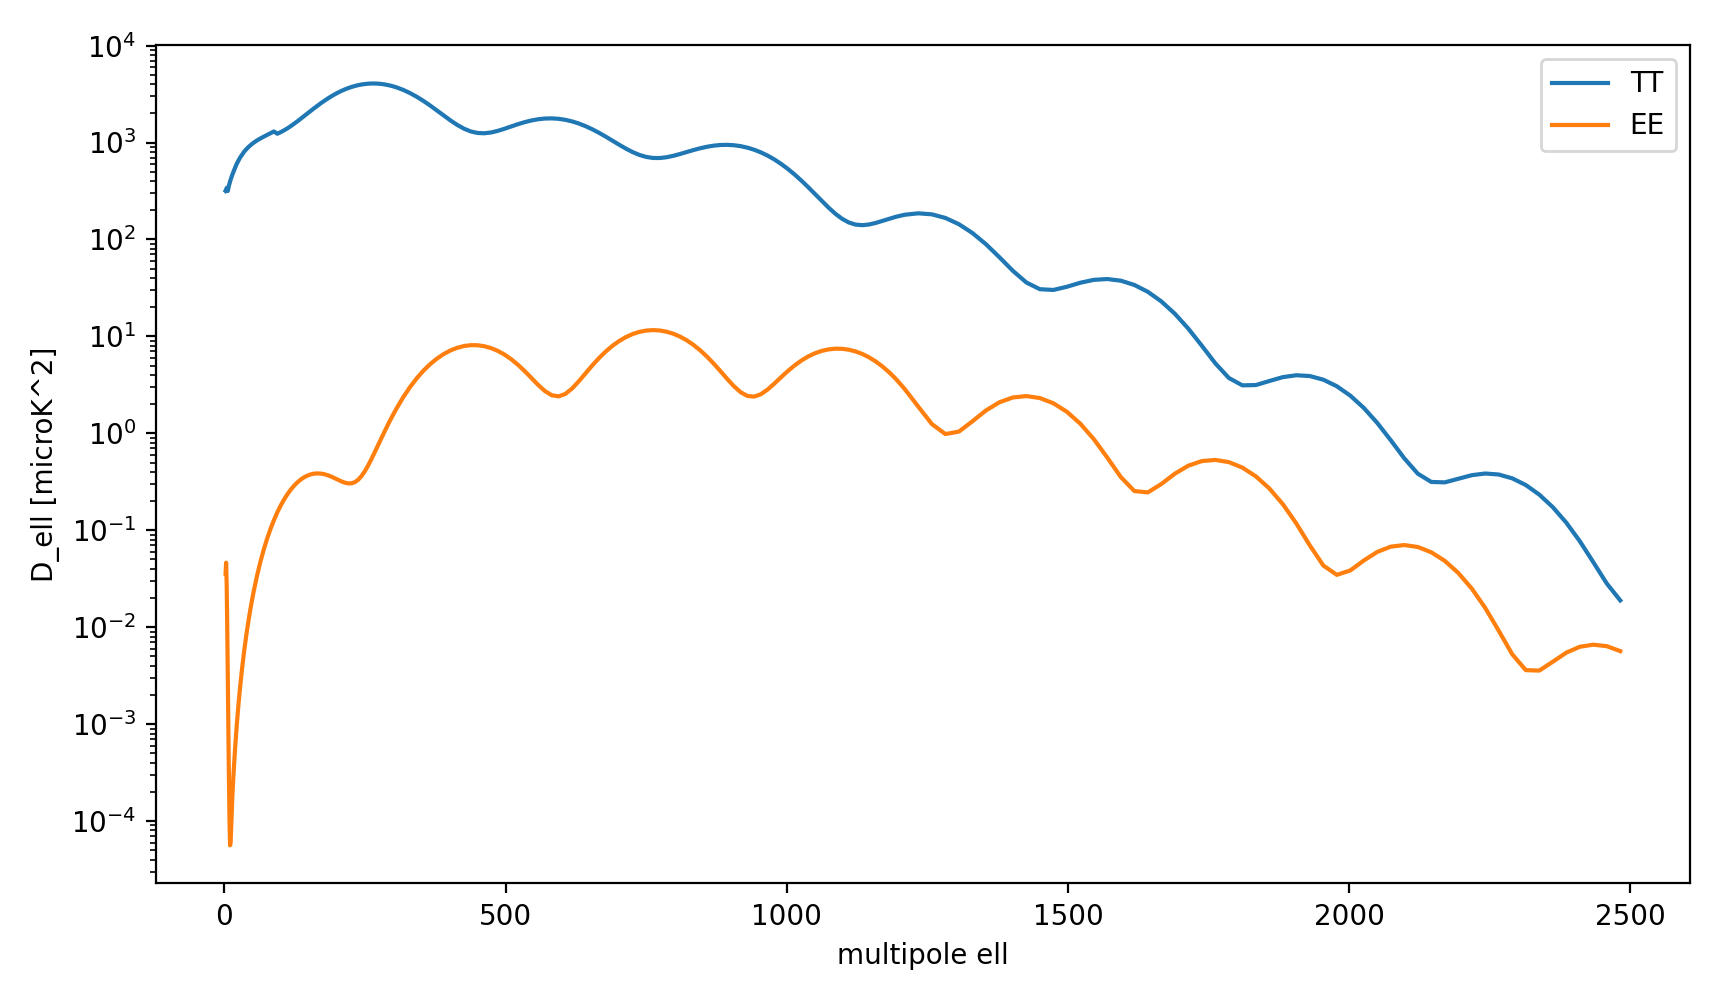
\includegraphics[width=0.88\linewidth]{figures/los/thermal_reionization_tt_ee.png}
\caption{Controlled temperature and scalar $E$-mode templates after effective recombination and reionization.}
\label{fig:trl-tt-ee}
\end{figure}

\begin{figure}[htbp]
\centering
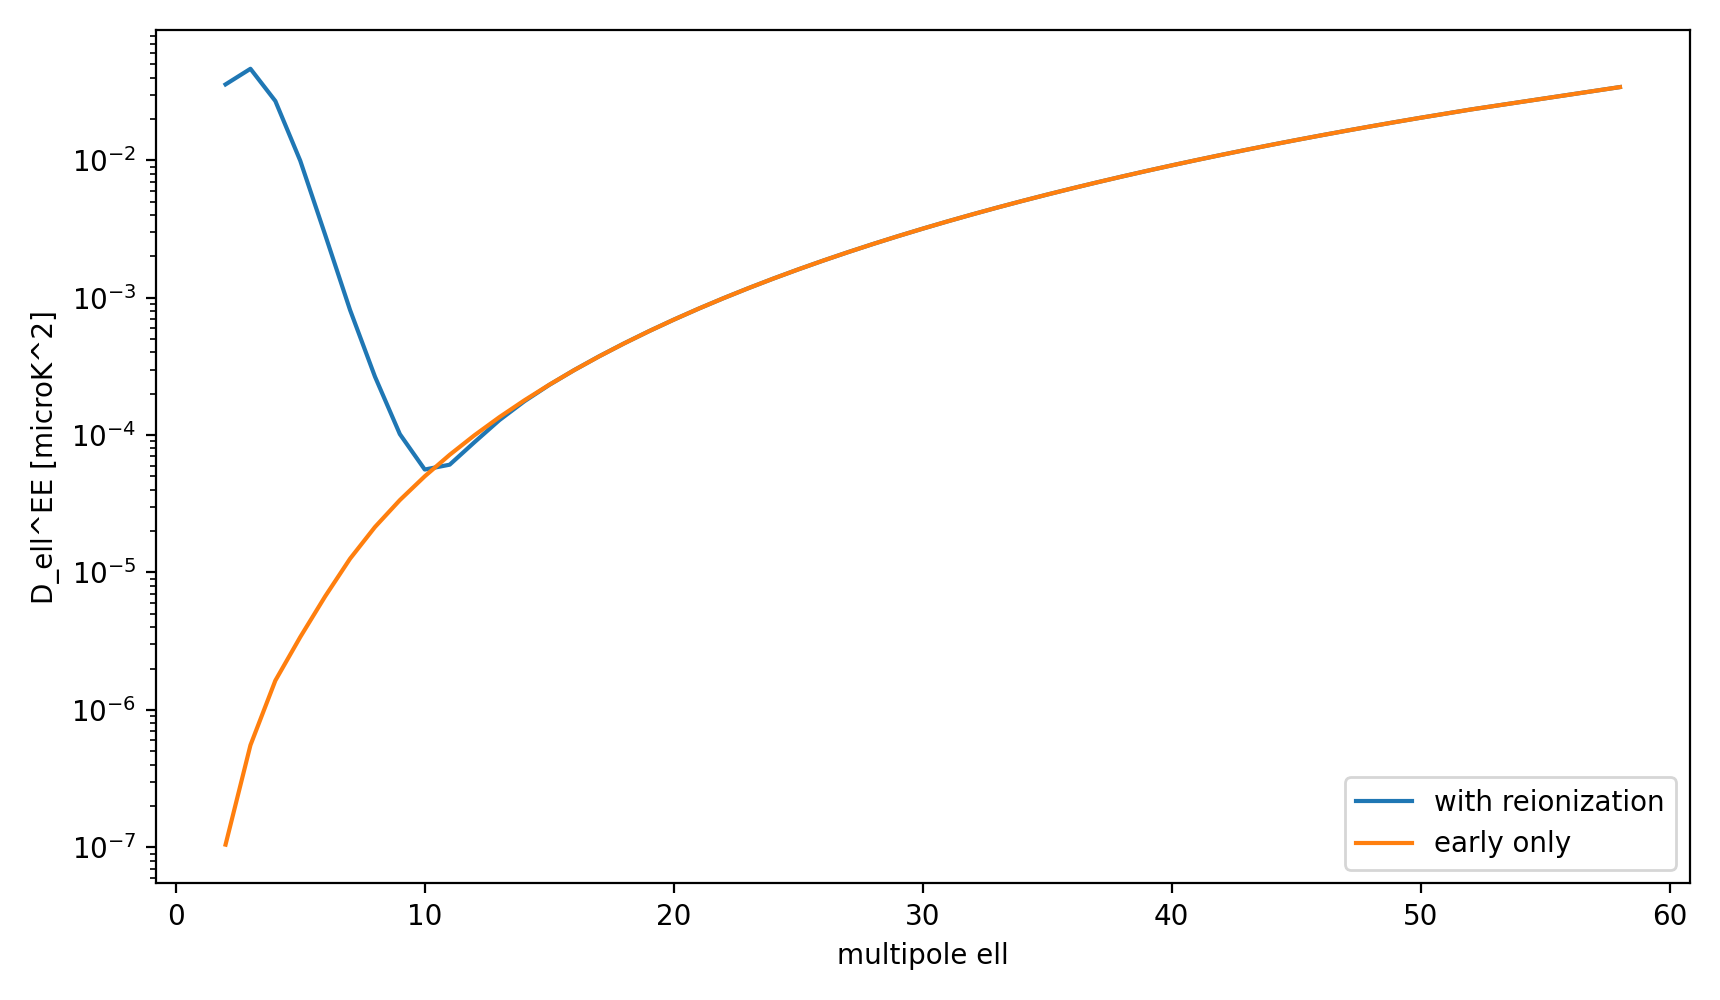
\includegraphics[width=0.84\linewidth]{figures/los/low_ell_ee_bump.png}
\caption{Reionization creates a low-multipole $E$-mode feature absent from the early-only source.}
\label{fig:trl-lowell-ee}
\end{figure}

\begin{figure}[htbp]
\centering
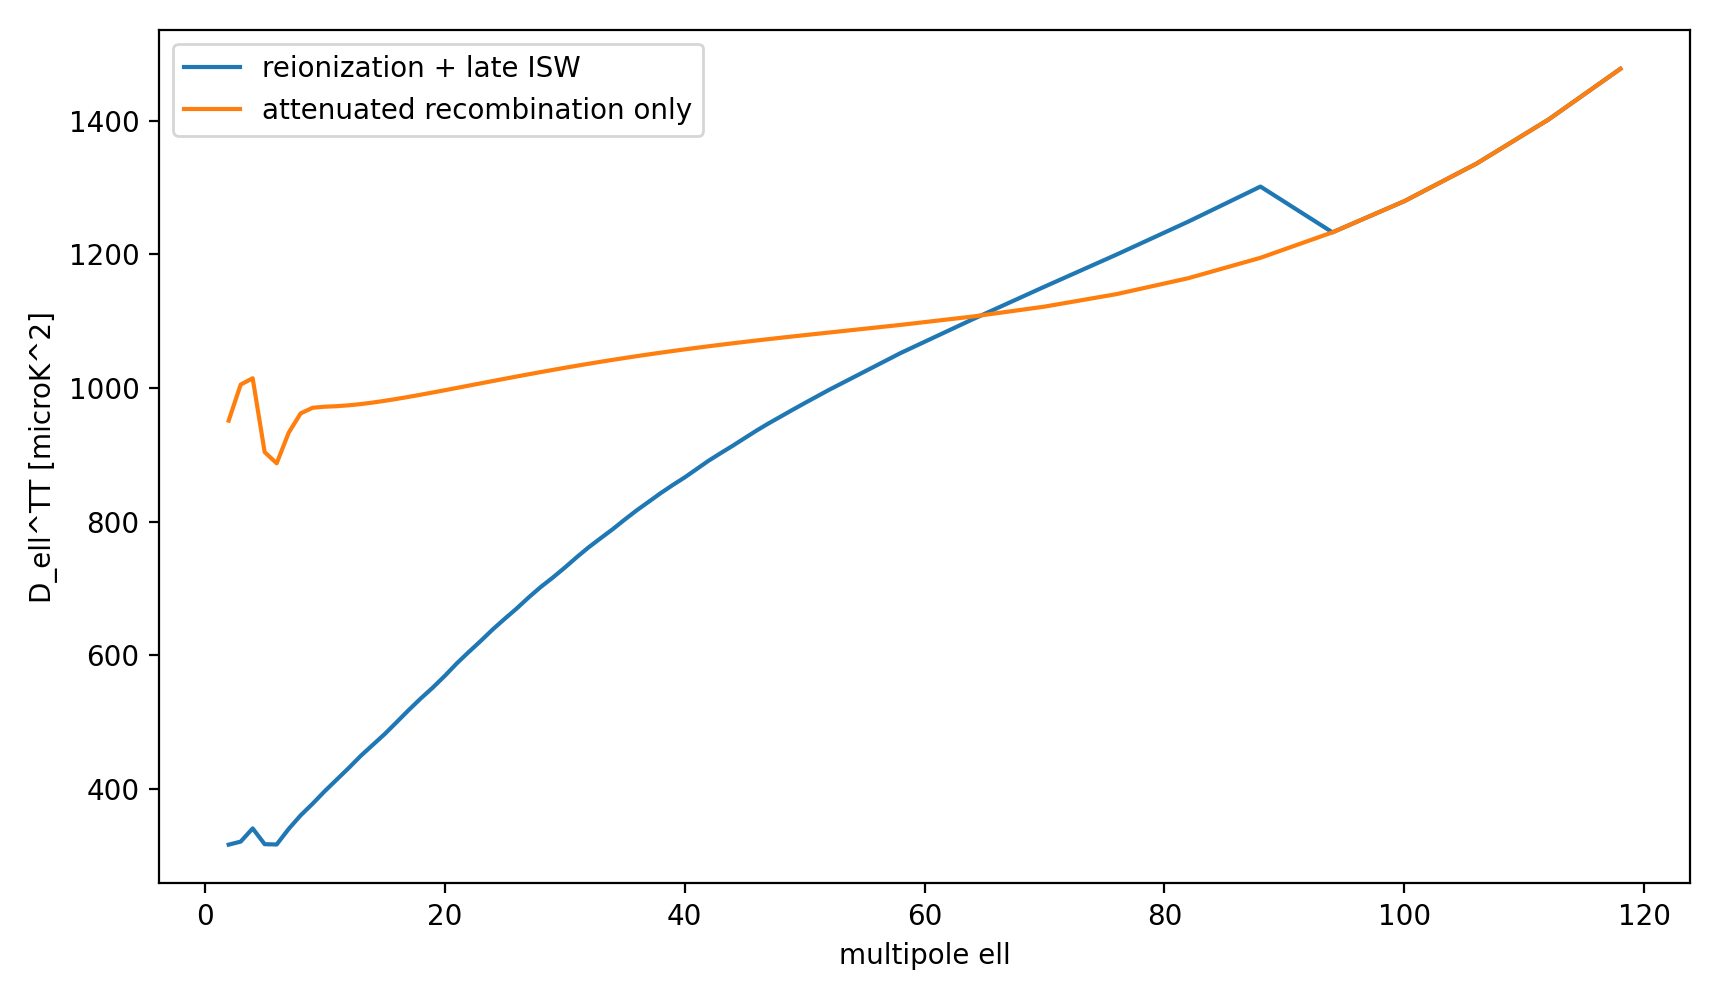
\includegraphics[width=0.84\linewidth]{figures/los/low_ell_tt_late_sources.png}
\caption{Late ISW and reionization modify the low-$\ell$ temperature source while leaving the acoustic regime effectively unchanged in this controlled projection.}
\label{fig:trl-lowell-tt}
\end{figure}

\begin{figure}[htbp]
\centering
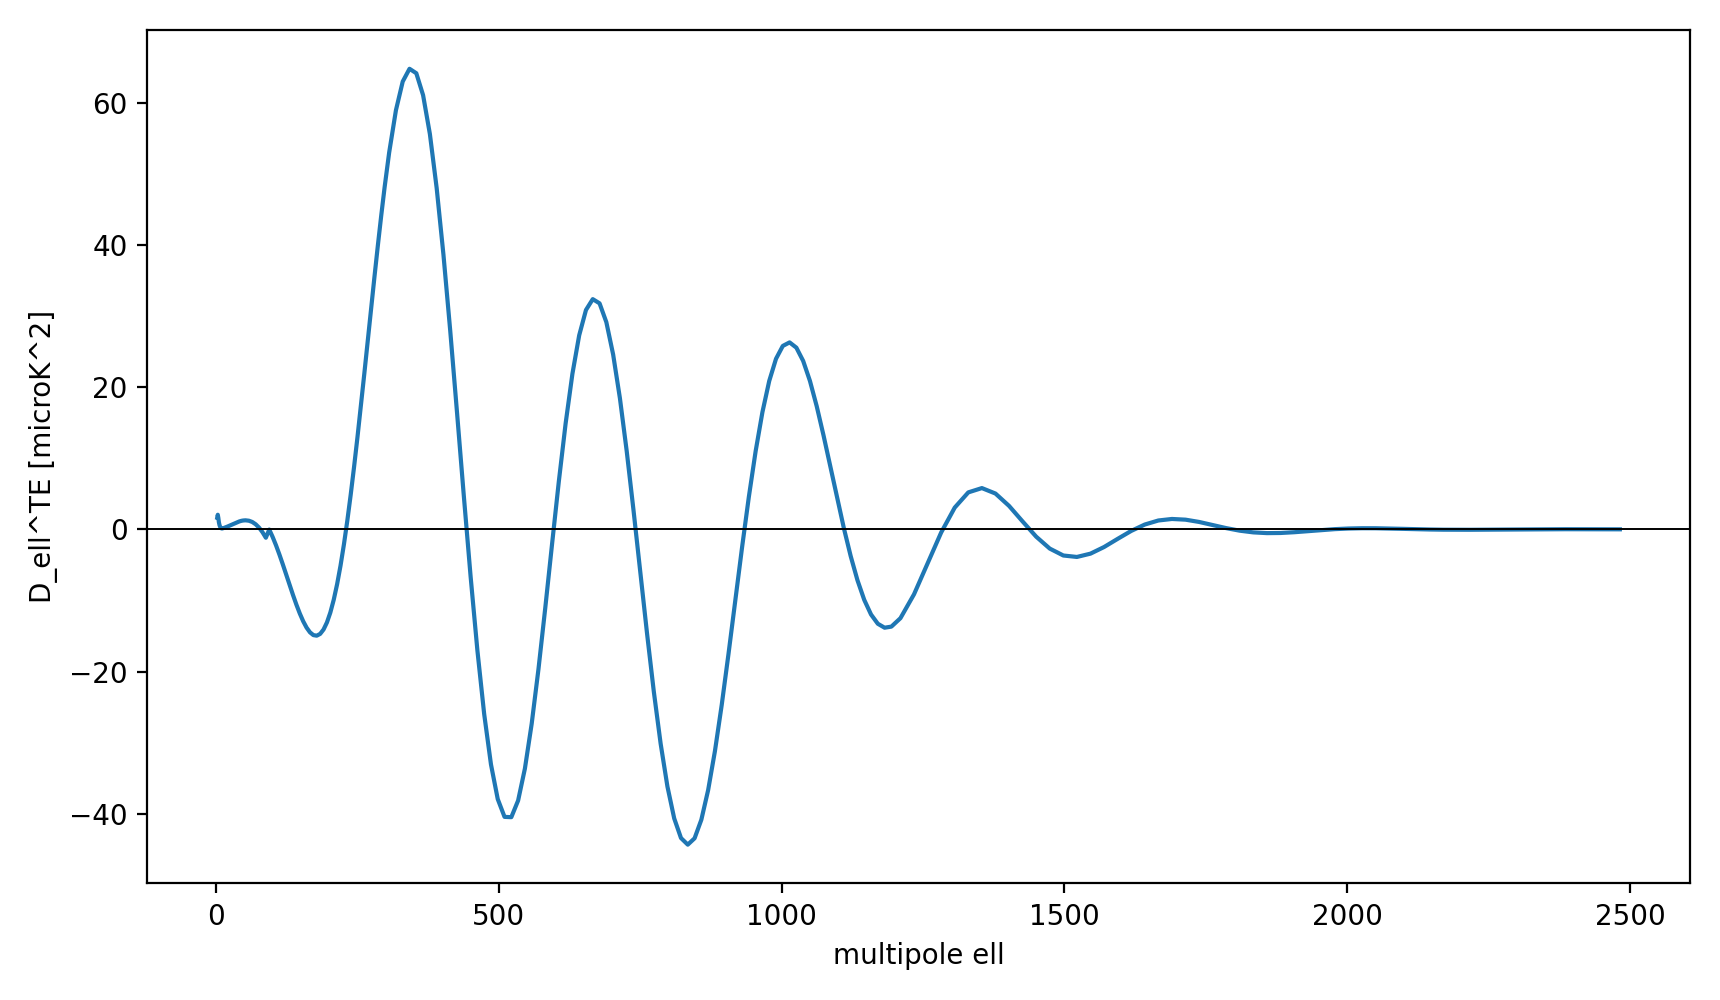
\includegraphics[width=0.88\linewidth]{figures/los/thermal_reionization_te.png}
\caption{Controlled TE template with alternating correlation sign across the acoustic structure.}
\label{fig:trl-te}
\end{figure}

\section{Projection convergence and deterministic audit}

The main projection uses 3350 global wavenumber nodes after combining logarithmic low-$k$ sampling with a linear oscillatory grid.  A 4500-node reference calculation was performed at selected multipoles.

\begin{table}[htbp]
\centering
\begin{tabular}{lrr}
\toprule
control & measured maximum & acceptance bound\\
\midrule
TT selected-grid discrepancy & $1.20461\times10^{-2}$ & $6\times10^{-2}$\\
EE selected-grid discrepancy & $4.42685\times10^{-2}$ & $6\times10^{-2}$\\
TE correlation discrepancy & $7.86181\times10^{-3}$ & $6\times10^{-2}$\\
acoustic TT discrepancy & $1.45217\times10^{-5}$ & $5\times10^{-2}$\\
\bottomrule
\end{tabular}
\caption{Main-to-fine projection convergence.}
\label{tab:trl-convergence}
\end{table}

\begin{figure}[htbp]
\centering
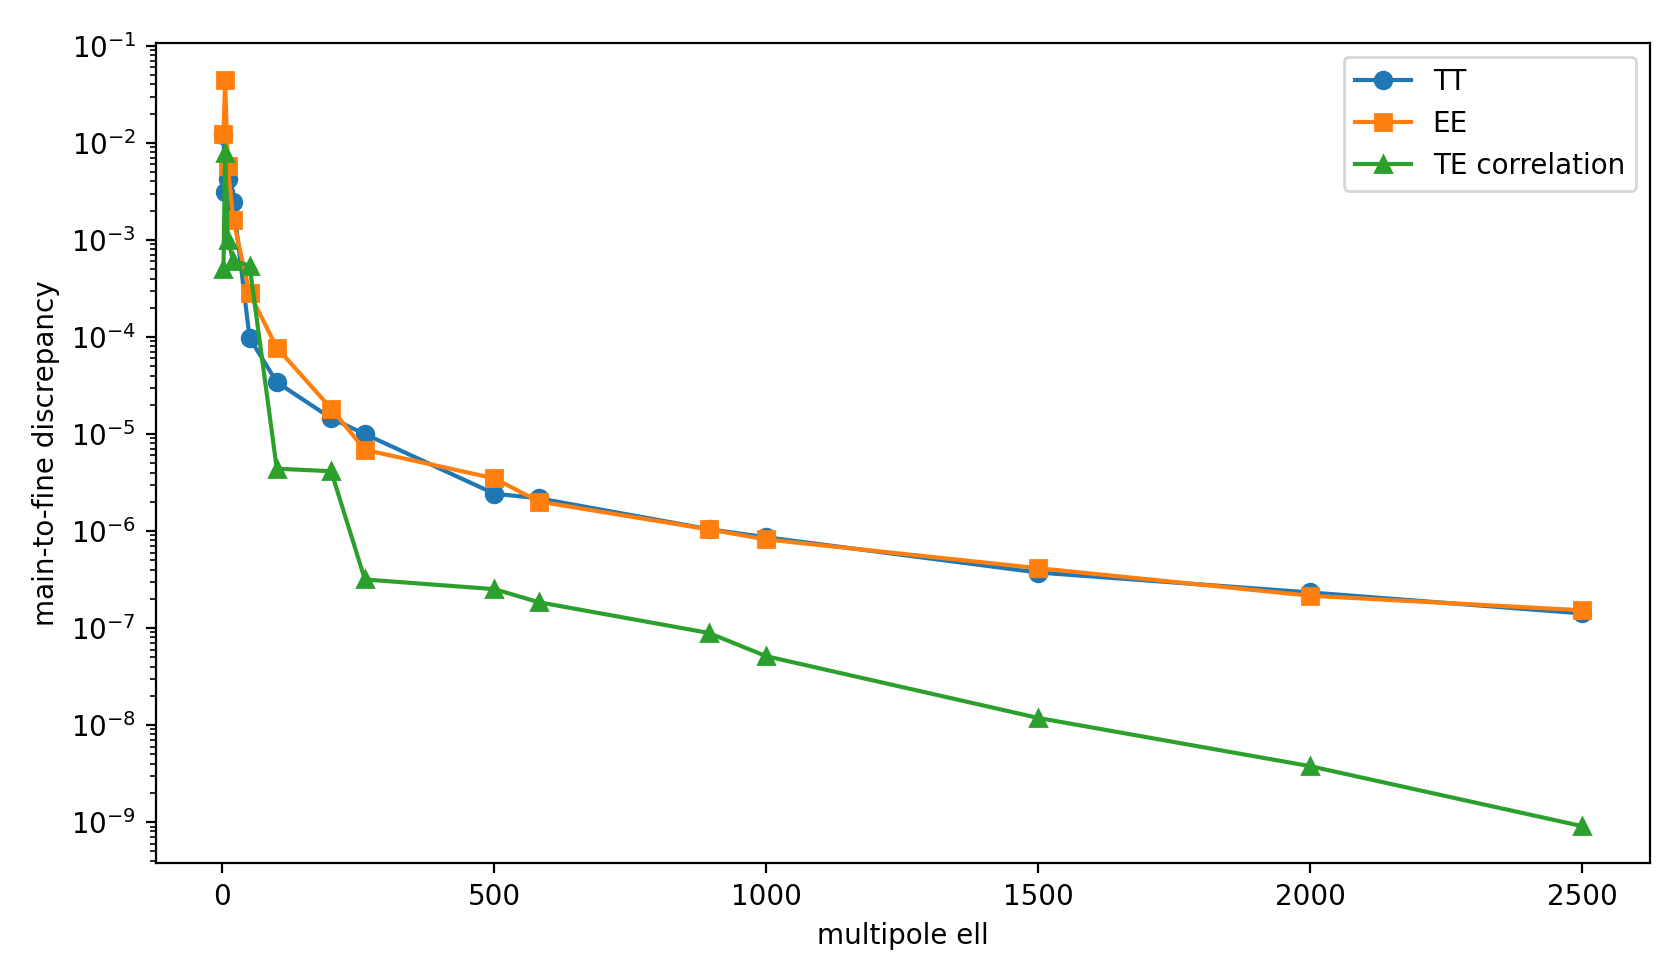
\includegraphics[width=0.82\linewidth]{figures/los/projection_convergence.png}
\caption{Selected-multipole convergence under global wavenumber-grid refinement.}
\label{fig:trl-convergence}
\end{figure}

The main deterministic suite records
\begin{equation}
\boxed{20\ {\rm PASS},\qquad0\ {\rm FAIL},}
\label{eq:trl-main-audit}
\end{equation}
and the independent projection-refinement suite records
\begin{equation}
\boxed{4\ {\rm PASS},\qquad0\ {\rm FAIL}.}
\label{eq:trl-convergence-audit}
\end{equation}
The combined result is
\begin{equation}
\boxed{24\ {\rm PASS},\qquad0\ {\rm FAIL}.}
\label{eq:trl-total-audit}
\end{equation}

\section{Closure ledger}

\begin{center}
\small
\begin{tabular}{p{0.43\linewidth}p{0.21\linewidth}p{0.28\linewidth}}
\toprule
statement & status & boundary\\
\midrule
effective Peebles hydrogen history & closed controlled & three-level approximation\\
controlled helium electron counting & closed conditional & smooth transition model\\
reionization optical depth & calibrated & $\tau_{\rm re}$ remains an input\\
recombination and reionization visibility & closed controlled & declared background\\
single-clock production matching & proved at leading order & no independent modulation\\
independent modulation response & derived & linear response\\
late ISW source sign & corrected & stated Newtonian-gauge convention\\
late time-resolved ISW projection & closed controlled & linear potential growth\\
finite-width recombination projection & closed controlled & central-shell approximation\\
low-$\ell$ reionization polarization & demonstrated & effective source reconstruction\\
precision multilevel H/He recombination & open & atomic kinetics\\
reionization redshift from astrophysics & open & source population\\
full recombination-time LOS integral & open & shell approximation retained\\
CMB lensing remapping & open & nonlinear structure\\
joint likelihood and posterior & open & data interface\\
\bottomrule
\end{tabular}
\end{center}

\section{Synthesis and scope}

This chapter closes three previously separate gaps:
\begin{equation}
\boxed{
\begin{gathered}
\text{production-surface adiabatic matching},\\
\text{effective recombination plus reionization},\\
\text{corrected late line-of-sight temperature and polarization sources}.
\end{gathered}}
\label{eq:trl-closed-chain}
\end{equation}
It also separates a robust statement from a model input.  A single-clock production event is adiabatic at leading gradient order, while an independent modulation field generates a calculable level-dependent entropy response.  The reionization optical depth is calibrated rather than predicted.

